\documentclass[11pt]{article}
\usepackage[a4paper,margin=27mm]{geometry}
\usepackage{amsmath,amssymb,amsthm,mathtools,booktabs,longtable}
\usepackage{tikz}
\usetikzlibrary{arrows.meta,calc,positioning,decorations.pathreplacing}
\usepackage[hidelinks]{hyperref}
\newtheorem{theorem}{Theorem}[section]
\newtheorem{proposition}[theorem]{Proposition}
\newtheorem{lemma}[theorem]{Lemma}
\newtheorem{corollary}[theorem]{Corollary}
\theoremstyle{definition}\newtheorem{definition}[theorem]{Definition}
\theoremstyle{remark}\newtheorem{remark}[theorem]{Remark}
\newcommand{\Hh}{\mathbb H}
\newcommand{\R}{\mathbb R}
\newcommand{\ip}[2]{\langle #1,#2\rangle}
\newcommand{\nuu}{\nu}
\newcommand{\Pthree}{P_3}
\newcommand{\Dthree}{D_3}
\newcommand{\Qeight}{Q_8}
\newcommand{\Rseven}{R_7}
\newcommand{\bin}[2]{\binom{#1}{#2}}
\newcommand{\file}[1]{\texttt{\detokenize{#1}}}
\tikzset{finite/.style={circle,draw,fill=black,inner sep=2.2pt},
 ideal/.style={circle,draw,fill=white,inner sep=2.7pt},
 move/.style={-{Stealth[length=2mm]},thick,blue!65!black},
 wall/.style={thick}, faint/.style={dashed,gray},
 every picture/.style={line cap=round,line join=round}}
\title{Opposition transport at mixed right-angled hyperbolic corners}
\author{Research manuscript}
\date{18 October 2026}
\begin{document}
\maketitle
\begin{abstract}
Actual opposite vertices in small three-dimensional faces give a finite
undirected transport graph on the finite vertices of a right-angled
hyperbolic polytope. We prove that a polytope whose every three-face has
facet-plus-cusp sum at most ten has dimension at most eight. A second
dimension-eight statement permits sum eleven but requires that no edge
join two finite vertices. Both hypotheses are essential to the arguments.
In dimension twelve a reciprocal transport estimate gives a positive
fraction of larger carriers, with total excess at least \(f/5390\),
where \(f\) is the finite-vertex count.
We also prove a component exit theorem, exact symmetric-quadrilateral
moves, and universal incidence bounds for their missing carriers.
These results do not improve the unconditional mixed dimension ceiling
twelve. Their geometric proofs are written arguments; two specified
finite arithmetic steps have separate exact checkers. No full Lean
formalization is asserted.
\end{abstract}

\section{Scope and conventions}
Let \(P\subset\Hh^n\) be a finite-volume right-angled polytope. In Lorentz
space of signature \((n,1)\), finite points are future unit vectors of
square \(-1\). Every facet has an outward unit spacelike normal \(r\);
the corresponding inequality is \(\ip{x}{r}\le0\). At a finite vertex
\(q\), its \(n\) incident normals \(n_1,\ldots,n_n\) are orthonormal.
Direction \(i\) means the edge obtained by omitting the wall \(n_i\).
An ideal point is represented by a future null ray. All equalities
between null vectors below use the particular displayed representatives.

For a three-face \(F\), write \(p(F),c(F),s(F)\) for its finite vertices,
cusps, and polygon facets, and put \(\nuu(F)=s(F)+c(F)\).
The letter \(f\) denotes the number of finite vertices of \(P\), and
\(a_j\) its number of \(j\)-faces. A \emph{bad triangle} means a
two-face with one finite and two ideal vertices. This descriptive name
does not indicate that such a face is forbidden.

The unconditional mixed ceiling remains \(n\le12\), as in the current
repository bounds table. This paper proves necessary conditions in
that range and two theorems with additional hypotheses. It does not
claim an example in dimension twelve, a universal bound eleven, or a
classification of all corner graphs. The entirely ideal dimension
problem is separate.

The geometric background used here is the usual acute-wall property of
Coxeter polytopes, the orthant link at a finite right-angled vertex,
the rectangular link at a three-dimensional cusp, and the elementary
incidence properties of convex polytopes; see also~\cite{PV}. We give
the small-face and transport arguments explicitly. The only finite
arithmetic verifications are the nine quadratic-field rows in
Table~\ref{tab:radical} and the precisely defined rational enclosure in
Lemma~\ref{lem:interval}. Their saved evidence and independent written
reviews are identified in the proof map.

\section{Actual walls and the small three-faces}
\subsection{Projection and the normal-product gap}
\begin{lemma}\label{lem:projection}
Mutually orthogonal actual facet normals determine their expected
finite intersection whenever that intersection is future timelike.
More generally, two distinct outward unit facet normals have product
zero or at most \(-1\).
\end{lemma}
\begin{proof}
Let \(x\) be a strict future timelike interior point. For orthonormal
normals \(u_\alpha\), its orthogonal projection is
\[
 x_0=x-\sum_\alpha\ip{x}{u_\alpha}u_\alpha.
\]
The added coefficients are positive. Acuteness implies
\(\ip{x_0}{r}\le\ip{x}{r}<0\) for every other facet normal \(r\).
Moreover \(x_0^2=x^2-\sum_\alpha\ip{x}{u_\alpha}^2<0\) and
\(\ip{x_0}{x}<0\), so \(x_0\) has the required time orientation.
This proves actual feasibility, including strictness for the other walls.

For the second statement acuteness gives \(g=\ip{u}{v}\le0\).
If \(-1<g<0\), the Gram matrix
\[
 G=\begin{pmatrix}1&g\\g&1\end{pmatrix}
\]
is positive definite with entrywise nonnegative inverse. With
\(b=(\ip{x}{u},\ip{x}{v})^T<0\), put
\(x_0=x-[u\ v]G^{-1}b\). Both added coefficients are positive,
\(x_0^2=x^2-b^TG^{-1}b<0\), and all other wall inequalities are
strict as before. Thus the two walls form an actual ridge with a
nonright dihedral angle, a contradiction. Positive products between
distinct outward normals are already excluded by acuteness.
\end{proof}

A useful companion observation is that a future null sum of actual
outward normals is feasible against every other wall by acuteness.
The finitely many summand walls must also be checked; we do so whenever
we use this observation.

\subsection{Triangles and their opposite finite vertices}
Define \(G_q\) on the \(n\) incident directions at \(q\) by putting
\(ij\in E(G_q)\) exactly when the corresponding two-face is a bad
triangle. Its ideal endpoints and third wall are
\begin{equation}\label{eq:badwall}
 u_i=q-n_i,\qquad u_j=q-n_j,\qquad m_{ij}=q-n_i-n_j.
\end{equation}
Conversely, if \(m_{ij}\) is an actual wall, these equations force the
bad triangle. Indeed \(u_i=n_j+m_{ij}\) and \(u_j=n_i+m_{ij}\)
are future null and feasible against every wall, including the three
selected walls. Those three inequalities enclose precisely this triangle
in the two-face plane, so convexity gives equality.

\begin{lemma}\label{lem:P3}
Every triangle \(S=\{i,j,k\}\) of \(G_q\) gives an actual three-face
\(\Pthree\), a triangular bipyramid with two finite and three ideal
vertices. Its opposite finite vertex is
\begin{equation}\label{eq:P3move}
 q_S=2q-n_i-n_j-n_k.
\end{equation}
Different triples at \(q\) give different opposite vertices.
\end{lemma}
\begin{proof}
The three normals \(m_{ij},m_{ik},m_{jk}\) are mutually orthogonal.
Together with the unchanged \(n_\ell\), \(\ell\notin S\), they
have the future unit intersection \eqref{eq:P3move}. To see strict
feasibility directly, write any other wall not through \(q\) as
\(r=a q-\sum c_\ell n_\ell\), where \(a>0\) and \(c_\ell\ge0\).
Its products with the three selected \(m\)'s imply
\(c_i+c_j,c_i+c_k,c_j+c_k\le a\), whence
\[
 \ip{r}{q_S}=-2a+c_i+c_j+c_k\le-\tfrac12a<0.
\]
The old three normals are also strict there. The six known walls in
the three-face plane enclose exactly
\(\operatorname{conv}(q,q_S,u_i,u_j,u_k)\). All five vertices are
feasible, so this is the whole three-face. The coordinate expression
in \eqref{eq:P3move} also proves distinctness of the opposites.
\end{proof}

\begin{figure}[ht]
\centering
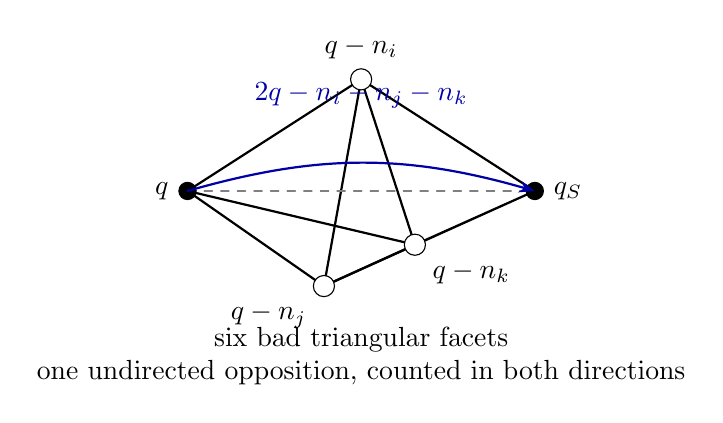
\begin{tikzpicture}[scale=1.05]
 \coordinate(q) at (-2.1,0); \coordinate(p) at (2.1,0);
 \coordinate(a) at (0,1.35); \coordinate(b) at (-.45,-1.15);
 \coordinate(c) at (.65,-.65);
 \draw[wall] (q)--(a)--(p)--(b)--(q)--(c)--(p);
 \draw[wall] (a)--(b)--(c)--(a);
 \draw[faint] (q)--(p);
 \node[finite,label=left:\(q\)] at(q){};
 \node[finite,label=right:\(q_S\)] at(p){};
 \node[ideal,label=above:\(q-n_i\)] at(a){};
 \node[ideal,label=below left:\(q-n_j\)] at(b){};
 \node[ideal,label=below right:\(q-n_k\)] at(c){};
 \draw[move,bend left=16] (q) to node[above=16pt]{\(2q-n_i-n_j-n_k\)} (p);
 \node[align=center] at (0,-2)
 {six bad triangular facets\\one undirected opposition, counted in both directions};
\end{tikzpicture}
\caption{The actual \(\Pthree\) three-face. This is an incidence drawing,
not a metric projection. Filled vertices are finite; hollow vertices
are ideal. The dashed segment is the opposition move, not an edge of
the polytope.}
\label{fig:P3}
\end{figure}

\begin{lemma}[Attachment]\label{lem:attachment}
If two bad triangular facets of a right-angled three-polyhedron share
their ideal--ideal edge, the entire three-polyhedron is \(\Pthree\).
\end{lemma}
\begin{proof}
Let their shared null endpoints be \(u,v\), scaled so that their first
finite apex \(q_1\) has products \(-1\) with both. Its right angle gives
\(\ip{u}{v}=-1\). If \(n_1,n_2\) are the orthogonal outward normals of
the triangles, their finite apices have the forms
\[
 q_1=u+v-n_2,\qquad q_2=s u+s^{-1}v-n_1,\quad s>0.
\]
To obtain these forms, expand each apex in \(u,v\) and the other
triangle normal. The unit norm and the right angle at the apex force
the normal coefficient to be \(-1\) and the product of its two null
coefficients to be one. The four side normals are
\[
 u-n_2,\quad v-n_2,\quad su-n_1,\quad s^{-1}v-n_1.
\]
Two cross products are \(-s,-s^{-1}\); the normal-product gap forces
\(s=1\). The third ideal vertex \(w=u+v-n_1-n_2\) is future null
and equals \((u-n_1)+(v-n_2)\), so it is feasible, also against
the selected walls. The six walls enclose exactly
\(\operatorname{conv}(q_1,q_2,u,v,w)\), proving the claim.
\end{proof}

\subsection{The complete list at sum at most ten}
For a right-angled three-polyhedron the vertex degrees are three at
finite vertices and four at cusps. Euler therefore gives
\begin{equation}\label{eq:Euler3}
 p+2c=2s-4,\qquad p+4c=2\nuu-4.
\end{equation}
A polygon with \(u\) finite and \(v\) ideal vertices has area
\(\frac\pi2(u+2v-4)>0\). Its integer excess \(u+2v-5\) is
nonnegative, and summation gives
\begin{equation}\label{eq:facetexcess}
 \sum_{\text{polygons}}(u+2v-5)=s+2c-12\ge0.
\end{equation}
Also \(s\ge6\): equivalently \(p+6c\ge20\), and if \(s\le5\)
then \(p+2c\le6\) and \(c\le3\), making this impossible. At
\(s=6\), these identities give \(c\ge3\). There are \(24-2c\)
polygon corners, so at least \(2c\) of the six polygons are triangles;
thus \(c\le3\). All six are bad triangles and Lemma~\ref{lem:P3}
identifies \(\Pthree\), with \((s,c,p)=(6,3,2)\).

\begin{proposition}\label{prop:small}
The three-polyhedra with \(\nuu\le10\) have exactly the following
combinatorial data. No metric uniqueness of \(\Qeight\) is needed.
\[
\begin{array}{c|ccc|l|l}
 &s&c&p&\text{polygons}&\text{ideal-edge degrees at finite vertices}\\ \hline
 \Pthree&6&3&2&6\text{ bad triangles}&3,3\\
 \Qeight&8&2&8&8\text{ quadrilaterals of type }(3,1)&1,1,1,1,1,1,1,1\\
 \Rseven&7&3&4&3\text{ bad triangles},\,1\text{ ideal triangle},
 \,3\text{ quads }(3,1)&0,2,2,2
\end{array}
\]
\end{proposition}
\begin{proof}
Outside \(\Pthree\) one has \(s\ge7\), and \(s+2c\ge12\)
leaves only \((s,c)=(8,2),(7,3)\) when \(s+c\le10\).
In the first case every polygon has zero excess. A triangle would be
bad, and the polygon across its ideal--ideal edge would also have zero
excess and contain two ideal vertices, hence be bad. Attachment would
give \(\Pthree\), a contradiction. There are \(32\) polygon corners,
so all eight polygons are quadrilaterals, each with one cusp. No finite
vertex can have two ideal incident edges, since their common polygon
would have two cusps. There are eight finite--ideal edges and eight
finite vertices, so every such degree is one.

In the second case the total excess is one and there are \(24\)
polygon corners. Hence at least four polygons are triangular, at least
three of them bad. Bad triangles have distinct ideal--ideal edges by
attachment. A zero-excess polygon other than a bad triangle is a
\((3,1)\) quadrilateral or a finite pentagon and cannot contain such an
edge. Thus all three distinct edges must lie in the unique excess-one
polygon. There can be no fourth such edge, since there are only three
cusps. Of the possible excess-one types
\((0,3),(2,2),(4,1),(6,0)\), only the all-ideal triangle contains
these three edges. There are exactly three bad triangles, and the
other three polygons are quads.
There are six finite--ideal edges and hence three finite--finite
edges. A finite vertex of ideal degree three would force
\(\Pthree\), and a degree-two corner supports at most one bad triangle.
If all four degrees were positive, the possibilities
\((1,1,1,3)\) and \((1,1,2,2)\) would support fewer than three bad
triangles. There is therefore a degree-zero vertex. Its three finite
neighbors are the other three finite vertices, using all finite edges;
their ideal degrees are two.
\end{proof}

\begin{lemma}\label{lem:shortedge}
Every finite edge of \(\Rseven\) has length \(L\) with
\(\cosh L=\sqrt2\).
\end{lemma}
\begin{proof}
Let \(q\) be its degree-zero center, with normals \(n_1,n_2,n_3\).
The three leaves and their bad-triangle normals are
\[
 q_i=\cosh L_i\,q-\sinh L_i\,n_i,\qquad
 r_i=\sinh L_i\,q-\cosh L_i\,n_i.
\]
The sign of \(r_i\) is fixed by its outward orientation. Each pair
of bad triangles meets only at their common cusp on the all-ideal
triangle, so their normals are an opposite pair in its rectangular
link. Thus \(\ip{r_i}{r_j}=-1=-\sinh L_i\sinh L_j\).
The three positive sines all equal one.
\end{proof}

\section{A conditional dimension-eight theorem}
\begin{theorem}\label{thm:small8}
If every three-face of \(P\) has \(\nuu\le10\), then \(n\le8\).
\end{theorem}
\begin{proof}
Suppose \(n\ge9\). The small faces have finite vertices, so \(P\)
has at least one finite vertex. At a finite \(q\), let \(k\) of its
directions end at ideal vertices and let \(m=n-k\).
Every triple of ideal directions is \(\Pthree\), by
Proposition~\ref{prop:small}. Every finite edge has
\(\cosh L=\sqrt2\). If \(k\ge2\), combine it with two ideal
directions to obtain an \(\Rseven\) leaf. If \(k\le1\), combine
it with two other finite directions to obtain an \(\Rseven\) center.
Lemma~\ref{lem:shortedge} applies in both cases.

Use actual finite edges with weight one and actual \(\Pthree\)
oppositions with weight \(1/20\). These relations are undirected;
different triples give different opposites, and the reverse opposition
uses the same three-face. Hence the sum over all finite vertices of
their displacement vectors \(D(q)\) is zero. Put
\[
 \tau=\sqrt2-1,\quad C=\bin{k}{3},\quad
 d=\begin{cases}\bin{k-1}{2}&k\ge3,\\0&k<3.\end{cases}
\]
In the frame at \(q\),
\begin{equation}\label{eq:smallD}
 D(q)=Aq-\frac d{20}\sum_{\rm ideal}n_i-\sum_{\rm finite}n_j,
 \qquad A=m\tau+\frac C{20}>0.
\end{equation}
Its time-square minus spatial-square is
\begin{equation}\label{eq:Delta}
 \Delta=A^2-m-\frac{kd^2}{400}
 =m^2\tau^2+m\left(\frac C{10}\tau-1\right)
   +\frac{d^2k(k-9)}{3600}.
\end{equation}
For \(k\ge9\) the last term is nonnegative and
\((C/10)\tau-1\ge(42\sqrt2-47)/5>0\).
For \(k\le8\), \(m\ge9-k\); Table~\ref{tab:radical}
gives positive base values and positive first increments. Every later
increment increases by \(2\tau^2>0\). Thus \(\Delta\ge0\)
for all \(n\ge9\). The only null case in the \(k\ge9\) tail is
\(k=9,m=0\), and its time coefficient is \(21/5>0\).

Each \(D(q)\) is consequently nonzero future causal. For any fixed
future unit \(u\), \(-\ip{u}{D(q)}>0\); summing contradicts
\(\sum_qD(q)=0\). This proves the theorem.
\end{proof}

\begin{table}[ht]\centering
\begin{tabular}{ccll}\toprule
\(k\)&\(m\)&\(\Delta(k,m)\)&\(\Delta(k,m+1)-\Delta(k,m)\)\\\midrule
0&9&\(234-162\sqrt2\)&\(56-38\sqrt2\)\\
1&8&\(184-128\sqrt2\)&\(50-34\sqrt2\)\\
2&7&\(140-98\sqrt2\)&\(44-30\sqrt2\)\\
3&6&\(20279/200-(357/5)\sqrt2\)&\(379/10-(259/10)\sqrt2\)\\
4&5&\(1359/20-48\sqrt2\)&\(158/5-(108/5)\sqrt2\)\\
5&4&\(199/5-28\sqrt2\)&\(25-17\sqrt2\)\\
6&3&\(35/2-12\sqrt2\)&\(18-12\sqrt2\)\\
7&2&\(17/8-\sqrt2\)&\(21/2-(13/2)\sqrt2\)\\
8&1&\(-229/50+(18/5)\sqrt2\)&\(12/5-(2/5)\sqrt2\)\\
\bottomrule\end{tabular}
\caption{The complete finite arithmetic in Theorem~\ref{thm:small8}.
Every entry is positive, as can be checked by squaring its rational
parts with the indicated signs. The saved exact checker compares in
\(\mathbb Q(\sqrt2)\), without floating point.}
\label{tab:radical}
\end{table}

\begin{figure}[ht]
\centering
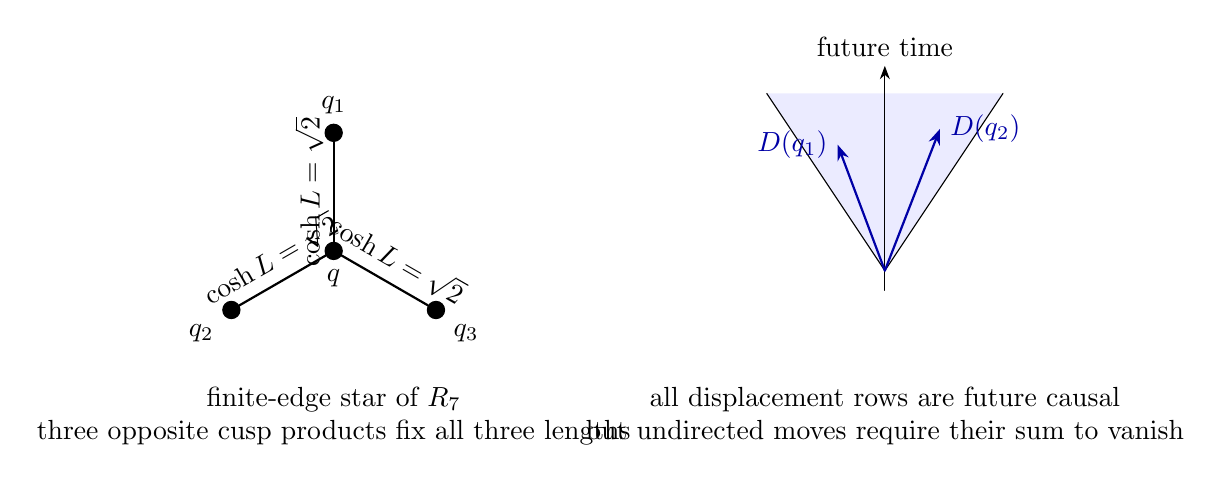
\begin{tikzpicture}
 \node[finite,label=below:\(q\)] (q) at (0,0){};
 \foreach \ang/\lab in {90/1,210/2,330/3}{
   \node[finite,label={\ang:\(q_{\lab}\)}] (p\lab) at (\ang:1.5){};
   \draw[wall] (q)--node[midway,sloped,above]{\(\cosh L=\sqrt2\)}(p\lab);
 }
 \node[align=center] at (0,-2.1){finite-edge star of \(\Rseven\)\\
 three opposite cusp products fix all three lengths};
 \begin{scope}[xshift=7cm,yshift=-.25cm]
  \fill[blue!8] (0,0)--(-1.5,2.25)--(1.5,2.25)--cycle;
  \draw[-{Stealth}] (0,-.25)--(0,2.6) node[above]{future time};
  \draw (-1.5,2.25)--(0,0)--(1.5,2.25);
  \draw[move] (0,0)--(-.6,1.6) node[left]{\(D(q_1)\)};
  \draw[move] (0,0)--(.7,1.8) node[right]{\(D(q_2)\)};
  \node[align=center] at (0,-1.85){all displacement rows are future causal\\
   but undirected moves require their sum to vanish};
 \end{scope}
\end{tikzpicture}
\caption{Two ingredients of the conditional obstruction. The left
panel is only the finite-edge subgraph of \(\Rseven\). The cone in the
right panel is schematic: the rigorous test is
\(A>0,\ A^2-\lVert b\rVert^2\ge0\) in the frame at each vertex,
followed by evaluation against one common future vector.}
\end{figure}

\section{A positive carrier-excess fraction in dimension twelve}
Define
\begin{equation}\label{eq:E}
 E=\sum_{F\ne\Pthree}(\nuu(F)-10).
\end{equation}
It is nonnegative by Proposition~\ref{prop:small}. If \(B\) counts
\(\Pthree\) faces and \(c_P\) counts cusps of \(P\), then in dimension
twelve incidence counting gives
\[
 E=B-10a_3+10a_2+28160c_P.
\]
Here each two-face lies in ten three-faces, and a cube of dimension
eleven has \(\bin{11}{2}2^9=28160\) two-faces, corresponding to
three-faces through a cusp.

\begin{theorem}\label{thm:fraction}
For \(n=12\), \(E\ge f/5390\). At least \(f/385\) finite vertices
are incident to a three-face with \(\nuu\ge11\).
\end{theorem}

Fix one future unit \(u\) for the whole polytope and put
\(H(q)=-\ip{u}{q}>0,\ g(q)=1/H(q)\).
Retain only actual finite edges of \(\cosh L=\sqrt2\), with weight
one, and actual \(\Pthree\) oppositions, with weight \(1/20\).
If \(d(q)\) is weighted degree and
\[
 R(q)=\sum_{q'\sim q}w(q,q')\frac{g(q')}{g(q)},
\]
undirected reciprocal pairing gives
\begin{equation}\label{eq:Schur}
 \sum_q(R(q)-d(q))\ge0.
\end{equation}
Call \(q\) \emph{small} if all its incident three-faces have sum at
most ten. At such a vertex, Theorem~\ref{thm:small8}'s local argument
identifies the whole selected row. In the frame at \(q\) put
\[
 p_i=-\frac{\ip{u}{n_i}}{H(q)},\qquad \sum_i p_i^2<1.
\]
Its energy ratios are \(\sqrt2-p_j\) for finite directions and
\(2-\sum_{i\in S}p_i\) for ideal triples \(S\). Replacing signs
by absolute values and increasing the norm to one enlarges the row.
All denominators remain positive, bounded below by
\(\sqrt2-1\) and \(2-\sqrt3\).

\subsection{A rational enclosure of the complete small row}
For a positive list \(r\), with mean \(\mu\) and \(r\ge a>0\),
the exact reciprocal identity gives
\begin{equation}\label{eq:moment1}
 \mathop{\rm av}\frac1r
 =\frac1\mu+\mathop{\rm av}\frac{(r-\mu)^2}{\mu^2r}
 \le\frac1\mu+\frac{\operatorname{Var}(r)}{a\mu^2}.
\end{equation}
Let \(k\) be the number of ideal directions, \(m=12-k\),
\(x=\sum_{\rm finite}p_j^2\), and write \(\sigma_f,\sigma_i\)
for the two nonnegative group sums. The finite contribution is at most
\begin{equation}\label{eq:finrow}
 \frac m{\mu_f}+\frac{x-\sigma_f^2/m}{a_f\mu_f^2},
 \quad \mu_f=\sqrt2-\sigma_f/m,\quad a_f=\sqrt2-\sqrt{x}.
\end{equation}
For \(k\ge3\), averaging uniformly over the ideal triples gives
\begin{equation}\label{eq:idealrow}
 \frac{\bin{k}{3}}{20}\left\{
 \frac1{\mu_i}+\frac{C_0(1-x-\sigma_i^2/k)}{a_i\mu_i^2}\right\},
 \quad C_0=\frac{3(k-3)}{k(k-1)},\
 \mu_i=2-\frac{3\sigma_i}k,\
 a_i=2-\sqrt{3(1-x)}.
\end{equation}
The variance formula follows by expanding a uniform three-subset sum:
each coordinate appears with probability \(3/k\), and each distinct
pair with probability \(6/[k(k-1)]\).

Here is the entire finite enclosure used in the theorem. For \(t\ge0\)
let \(L(t),U(t)\) be the adjacent multiples of \(10^{-7}\) enclosing
\(\sqrt t\), obtained by integer square root; use equality at an exact
grid square. Set
\[
 b_0=\frac{1414213562373095}{10^{15}}<\sqrt2.
\]
For a norm interval \([\ell,h]\) define a finite-group bound as follows
when \(m>0\):
\[
 a=b_0-U(h),\quad Q=h/m,\quad
 y_-=\frac{L(\ell)}m,\quad y_+=U(h/m),\quad
 y_*=\left[\frac{ab_0+2Q}{a+2b_0}\right]_{[y_-,y_+]},
\]
\begin{equation}\label{eq:certF}
 U_f=m\left\{\frac1{b_0-y_*}
       +\frac{Q-y_*^2}{a(b_0-y_*)^2}\right\}.
\end{equation}
Brackets denote clipping to the given interval. When \(k\ge3\) set
\[
 z=1-\ell,\quad a=2-U(3z),\quad
 y_-=\frac{L(1-h)}k,\quad y_+=U(z/k),\quad
 y_*=\left[\frac{6a+6C_0z}{9a+4kC_0}\right]_{[y_-,y_+]},
\]
\begin{equation}\label{eq:certI}
 U_i=\frac{\bin{k}{3}}{20}
 \left\{\frac1{2-3y_*}+
       \frac{C_0(z-ky_*^2)}{a(2-3y_*)^2}\right\}.
\end{equation}
Absent groups contribute zero.

\begin{lemma}[Finite rational enclosure]\label{lem:interval}
For \(1\le k\le11\), use the sixteen intervals
\([\ell,h]=[j/16,(j+1)/16]\), \(0\le j<16\).
For \(k=0\) use only \([1,1]\), and for \(k=12\) only \([0,0]\).
On all \(178\) resulting boxes the denominators above are positive and
\[
 m+\frac{\bin{k}{3}}{20}-(U_f+U_i)>\frac{125535}{10^6}>\frac18.
 \tag{\(*\)}
\]
Consequently every small vertex has \(R(q)\le d(q)-1/8\).
\end{lemma}
\begin{proof}
The finite verification of \((*)\) is rational: compute \(L,U\)
by integer square root, clip the two displayed rational critical
points, and compare by cross multiplication. These definitions specify
every box and every operation; the separate saved checker and
certificate record the minimum for each \(k\). This is the finite
arithmetic input of the lemma, not sampling of directions.

We justify why that finite input covers every real direction.
For the finite group
\(\sqrt x\le\sigma_f\le\sqrt{mx}\).
At an actual \(y=\sigma_f/m\), the inflated numerator
\(h/m-y^2\) is nonnegative. Decreasing the positive denominator
parameters to \(b_0,a\), and increasing \(x\) to \(h\), is therefore
a valid upper bound \emph{at that actual point}. Only after this
comparison do we enlarge its \(y\)-interval. The derivative of
\[
 \frac1{b-y}+\frac{Q-y^2}{a(b-y)^2}
\]
has the sign of \(ab+2Q-y(a+2b)\), so its maximum on the enlarged
interval is exactly \eqref{eq:certF}. The same argument for the ideal
group uses \(ky^2\le1-x\le z\) at actual points and the derivative
sign \(6a+6C_0z-y(9a+4kC_0)\), giving \eqref{eq:certI}.
Extra nonphysical points with negative variance numerator cause no
problem in maximization over a superset. Thus \((*)\) proves the
claimed bound over the entire sphere.
\end{proof}

\begin{proof}[Proof of Theorem~\ref{thm:fraction}]
At any nonsmall vertex the selected move lengths alone give
\[
 R(q)-d(q)\le12\sqrt2+11(1+\sqrt3)<48.
\]
For example \(\sqrt2<10/7,\sqrt3<7/4\) verify the last inequality.
If \(b\) vertices are nonsmall, \eqref{eq:Schur} gives
\(0\le-(f-b)/8+48b\), hence \(b\ge f/385\).

A three-face with \(\nuu\ge11\) has
\(p\le14(\nuu-10)\). At \(\nuu=11\),
\(s+2c\ge12\) gives \(s\le10\), and
\(p=4s-2\nuu-4\le14\). At \(\nuu\ge12\) use
\(p\le2\nuu-4\le14(\nuu-10)\).
Counting incidences with nonsmall vertices yields
\(b\le\sum_{\nuu\ge11}p\le14E\).
If \(f=0\) the assertion is immediate; otherwise these inequalities
prove both claims.
\end{proof}

The rational enclosure in this section is specific to dimension twelve.
It supplies neither a dimension-eleven fraction nor an exclusion of
twelve. In particular a small positive excess need not meet any later
global density target.

\section{What an actual opposition transports}
\subsection{The invariant and the cross edges}
Label the new incident normals after the move on
\(S=\{i,j,k\}\) by
\begin{equation}\label{eq:newnormals}
 n'_i=q-\sum_{h\in S\setminus\{i\}}n_h\quad(i\in S),
 \qquad n'_\ell=n_\ell\quad(\ell\notin S).
\end{equation}
These are the actual normals of Lemma~\ref{lem:P3}, with labels chosen
for comparison. Direct substitution gives
\begin{equation}\label{eq:cross}
 q_S-n'_i-n'_\ell=q-n_i-n_\ell
 \quad(i\in S,\ \ell\notin S).
\end{equation}
By the wall characterization \eqref{eq:badwall}, every cross edge of
\(G_q\) is preserved in both directions. The internal triangle is
also preserved. An edge between two unchanged directions \(a,b\)
instead requires the actual wall
\[
 2q-\sum_{i\in S\cup\{a,b\}}n_i.
\]
We do not infer this wall from a five-clique alone.

Let \(\Gamma\) be the finite graph on finite vertices of \(P\), with
one edge for each actual \(\Pthree\) opposition. Distinct triples
give distinct neighbors, so \(\deg_\Gamma(q)=t(G_q)\). The vector
\begin{equation}\label{eq:h}
 h=3q-\sum_{i=1}^n n_i,\qquad h^2=n-9,\quad \ip{h}{q}=-3,
\end{equation}
is constant on each connected component by \eqref{eq:newnormals}.
It is null at \(n=9\), and spacelike at \(n=10,11,12\).

At a small vertex \(G_q\) is \(K_k\) plus isolates, since every pair
of ideal directions lies in a small carrier and hence gives a bad
triangle. The three directions of any opposition arriving from such
a vertex are therefore true twins at its recipient: they form a
triangle with identical outside neighborhoods. Thus the number of
incoming small corners is at most
\begin{equation}\label{eq:twins}
 \sum_C\bin{|C|}{3},
\end{equation}
where \(C\) runs through the true-twin classes of the recipient graph.
An incoming complete corner uses three universal vertices.

\begin{figure}[ht]
\centering
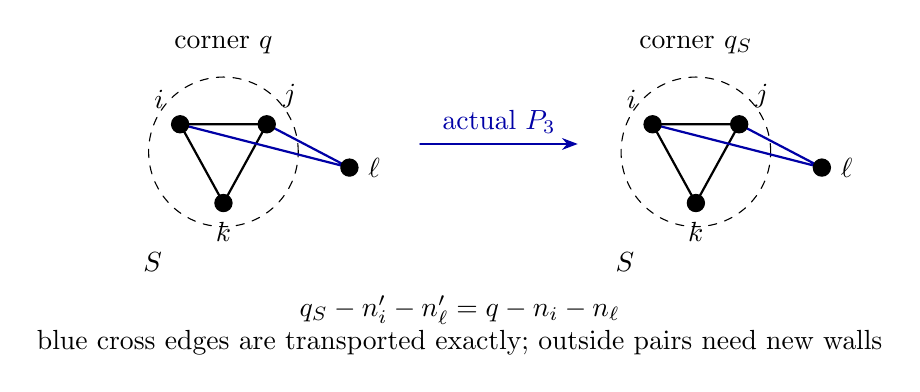
\begin{tikzpicture}
 \foreach \x/\lab in {0/q,6/{q_S}}{
  \begin{scope}[xshift=\x cm]
   \node[circle,draw,dashed,minimum size=19mm] at(0,.2){};
   \node at(0,1.55){corner \(\lab\)};
   \coordinate(a) at(-.55,.55);\coordinate(b) at(.55,.55);
   \coordinate(c) at(0,-.45);\coordinate(d) at(1.6,0);
   \draw[wall] (a)--(b)--(c)--(a);
   \draw[blue!65!black,thick] (a)--(d) (b)--(d);
   \node[finite,label=above left:\(i\)] at(a){};
   \node[finite,label=above right:\(j\)] at(b){};
   \node[finite,label=below:\(k\)] at(c){};
   \node[finite,label=right:\(\ell\)] at(d){};
   \node at(-.9,-1.2){\(S\)};
  \end{scope}
 }
 \draw[move] (2.5,.3)--node[above]{actual \(\Pthree\)}(4.5,.3);
 \node[align=center] at(3,-2)
 {\(q_S-n'_i-n'_\ell=q-n_i-n_\ell\)\\
 blue cross edges are transported exactly; outside pairs need new walls};
\end{tikzpicture}
\caption{Transport of corner-graph data. Dots here represent incident
directions, not hyperbolic vertices. A triple flip preserves the
cross edges, but it does not automatically complete the graph outside
the triple.}
\end{figure}

\subsection{A component cannot remain in the \(K_9\) region}
\begin{theorem}\label{thm:exit}
Every nontrivial component of \(\Gamma\) in dimensions \(9\) through
\(12\) contains a corner graph with no \(K_9\).
\end{theorem}
\begin{proof}
At a corner put \(t=t(G_q)\), and let \(b_i\) count its triangles
containing direction \(i\). The sum of all actual opposition
displacements is
\begin{equation}\label{eq:triD}
 D_\triangle(q)=tq-\sum_i b_i n_i,\qquad
 D_\triangle(q)^2=\sum_i b_i^2-t^2.
\end{equation}
If \(t>0\) and \(\sum b_i^2\le t^2\), this is nonzero future
causal. Undirected cancellation in a finite nontrivial component
therefore requires at least one corner with \(\sum b_i^2>t^2\).

We prove that a graph on at most twelve vertices containing \(K_9\)
never has this strict inequality. Choose a \(K_9\); it supplies
\(84\) triangles and incidence \(28\) at each of its nine vertices.
Let \(M\) count additional triangles, \(c_i\) their incidences at
the nine chosen vertices, \(d_j\) their incidences outside, and
\(O=\sum_jd_j\). There are at most three outside vertices, so
\[
 O\ge M,\quad \sum_i c_i=3M-O,\quad
 c_i\le3\cdot8+\bin32=27,\quad
 d_j\le L:=\min(M,55).
\]
The \(c_i\) bound separately counts one outside and one old vertex,
or two outside vertices. Expanding the squares gives
\begin{align*}
 \sum b_i^2-t^2
 &=\sum c_i^2+\sum d_j^2-M^2-56O\\
 &\le27(3M-O)+LO-M^2-56O\\
 &\le M(L-M-2)\le-2M.
\end{align*}
The penultimate step uses \(L<83\) and \(O\ge M\).
For \(M=0\) equality is zero. Thus every \(K_9\)-containing
corner gives a causal displacement, which proves the theorem.
\end{proof}

This is an exit statement about an actual connected graph, rather than
a statement about a formal distribution of clique counts. It gives no
uniform fraction of exit vertices. In particular a very long component
with few exit vertices is not excluded by this argument.

\subsection{A reciprocal-square cap and a boundary inequality}
The remainder of this subsection is specifically in dimension twelve.
By \eqref{eq:h}, choose a future null \(z\perp h\) separately on
each opposition component, and put
\[
 E_z(q)=-\ip{z}{q}>0,\quad
 p_i=-\frac{\ip{z}{n_i}}{E_z(q)}.
\]
Then \(\sum p_i=3,\ \sum p_i^2=1\).
For all \(220\) formal triple flips, set
\[
 r_S=\frac{E_z(2q-\sum_{i\in S}n_i)}{E_z(q)}
      =2-\sum_{i\in S}p_i.
\]
The formal point is future unit timelike even when it is not a vertex
of \(P\); we use it only to upper-bound a positive sum over actual
neighbors. Write \(x_i=p_i-1/4,\ \mu=5/4\), and
\(d_S=-\sum_{i\in S}x_i\). Then
\(\sum x_i=0,\ \sum x_i^2=1/4\), and zero-sum Cauchy--Schwarz gives
\[
 |d_S|\le3/4,\qquad 1/2\le r_S\le2.
\]
Uniform averaging over triples, by their repeated-index patterns,
gives
\begin{align*}
 \mathop{\rm av}d&=0,&
 \mathop{\rm av}d^2&=9/176,\\
 \mathop{\rm av}d^3&=-(27/220)\sum x_i^3,&
 \mathop{\rm av}d^4&=3/440-(3/220)\sum x_i^4\le3/440.
\end{align*}
For example the inclusion probabilities for one, two and three fixed
indices are \(1/4,1/22,1/220\). The cubic power-sum coefficient
is \(1/4-3/22+2/220=27/220\). The fourth coefficients are
\(-3/220\) for \(\sum x_i^4\) and \(6/55\) for
\((\sum x_i^2)^2\). Also \(\lvert\sum x_i^3\rvert\le1/8\).
The exact identity
\[
 \frac1{r^2}=\frac1{\mu^2}-\frac{2d}{\mu^3}
 +\frac{3d^2}{\mu^4}-\frac{4d^3}{\mu^5}
 +\frac{d^4(4r+\mu)}{\mu^5r^2}
\]
has remainder multiplier \(4/r+\mu/r^2\le13\) for \(r\ge1/2\).
It follows that
\[
 \mathop{\rm av}r^{-2}
 \le\frac{16}{25}+\frac3{\mu^4}\frac9{176}
 +\frac4{\mu^5}\frac{27}{1760}
 +\frac{13}{\mu^5}\frac3{440}
 =\frac{129248}{171875}.
\]
With \(g(q)=E_z(q)^{-2}\), positivity and restriction to actual
neighbors prove the row bound
\begin{equation}\label{eq:A}
 \sum_{q'\sim_\Gamma q}\frac{g(q')}{g(q)}
 \le A:=\frac{516992}{3125}=165.43744.
\end{equation}
Isolated vertices need no choice of \(z\). Every actual ratio is in
\([1/4,4]\). Hence, if \(W\) is any vertex subset of a component,
reciprocal pairing on its internal edges gives
\begin{equation}\label{eq:boundary}
 2e(W)+\tfrac14|\partial W|\le A|W|.
\end{equation}
Summing over components is legitimate because their choices of \(z\)
are separate. In particular \(2B\le A f_{\Pthree}\), where
\(f_{\Pthree}\) counts finite vertices incident to some \(\Pthree\).

For a concrete application let \(W\) consist of corners with
\(G_q=K_{12}\) minus three disjoint edges, the multipartite pattern
with six singleton and three doubled parts. Its degree is \(190\).
Every opposition from such a corner again has all directions ideal:
each outside direction retains at least two cross edges. Its only
true-twin class of size at least three is the class of six universal
vertices. Thus \eqref{eq:twins} allows at most \(20\) edges from
each such corner to complete corners. Since
\(190|W|=2e(W)+|\partial W|\), \eqref{eq:boundary} implies
\[
 |\partial W|\ge\frac{102344}{3125}|W|.
\]
At least \(39844|W|/3125\) of those edges reach further
noncomplete, all-ideal-direction corners outside \(W\).
Actual graph support restricted to the empty graph, \(K_{12}\),
and this single multipartite pattern is therefore impossible if \(W\)
is nonempty. Clique moments alone do not encode this exclusion.

The displayed cap is the separately reviewed reciprocal-square input.
A later direction-polynomial note sharpens its numerical value, but
that change is not needed for these stated support constants. Neither
cap yields a dimension improvement.

\subsection{Finite-edge support has a capacity constraint}
Call a finite--finite edge \emph{clean} if all its three-face carriers
have sum at most ten. Every two-face through it is a \((3,1)\)
quadrilateral, so it exchanges finite and ideal status in every other
direction between its endpoints. Consequently \(k'=n-1-k\).
Moreover a pair of new ideal directions and this edge is an
\(\Rseven\) leaf, so those directions are a bad pair. Thus each
endpoint graph is complete on its ideal directions, with isolates
elsewhere.

Let \(v_0\) count empty corner graphs, let \(v_j\) count graphs
\(K_j\) plus isolates for \(j\ge3\), and let \(Y(q)\) count
three-faces with \(\nuu\ge11\) incident to \(q\). Then
\begin{equation}\label{eq:edgecap}
 (n-1)v_0\le v_{n-1}+2v_{n-2}
             +3\sum_{G_q\ {\rm empty}}Y(q)\qquad(n\ge5).
\end{equation}
Indeed an empty corner with \(k\le1\) has at least \(n-1\)
finite edges; clean ones end at the two indicated types, whose finite
edge capacities are one and two. Each unclean edge uses a large
three-face, with at most three such edges at \(q\) per carrier.
If an empty corner has \(k\ge2\), every triple with at least two
ideal directions is large. Thus
\[
 Y(q)\ge\bin{k}{3}+(n-k)\bin{k}{2}\ge n-2.
\]
The last expression is nondecreasing in integer \(k\), with successive
difference \(k(n-k-1)\); its value at \(k=2\) is \(n-2\).
This also pays \((n-1)\) per such vertex by the final term in
\eqref{eq:edgecap}.

For \(n=12\), a corner of the preceding nine-part pattern has exactly
\(30\) large carriers: precisely its triples containing a missing
pair. The finite-vertex bound used in Theorem~\ref{thm:fraction},
and disjointness of these corners from empty corners, give
\[
 42E\ge11v_0-v_{11}-2v_{10}+90|W|.
\]
This is an incidence budget, not a proof that the right side always
forces a contradiction.

\section{Symmetric quadrilaterals with no global carrier hypothesis}
\subsection{The actual move and its rigidity}
\begin{lemma}\label{lem:quad}
For directions \(i,j\) at a finite corner \(q\), put
\begin{equation}\label{eq:quad}
 R_i=2q-n_i-2n_j,\quad R_j=2q-2n_i-n_j,\quad
 q_{ij}=3q-2n_i-2n_j.
\end{equation}
If \(R_i,R_j\) are actual facet normals, the corresponding two-face
is a quadrilateral with opposite finite vertices \(q,q_{ij}\)
and ideal vertices \(q-n_i,q-n_j\). Its finite diagonal has
\(\cosh L=3\). Conversely a two-face of this vertex type and this
diagonal length has exactly these side normals.
\end{lemma}
\begin{proof}
The new normals and the unchanged \(n_\ell\) are orthonormal.
Their future unit intersection is \(q_{ij}\), actual by
Lemma~\ref{lem:projection}. The null endpoints are feasible because
\[
 q-n_i=(n_j+R_j)/2,\qquad q-n_j=(n_i+R_i)/2.
\]
The four selected inequalities enclose precisely the displayed
quadrilateral in the two-face plane.

For the converse, a general such quadrilateral has opposite finite
vertex \(p=a q-c n_i-d n_j\), with \(a>1,c,d>0\).
Its right angle and unit norm give
\[
 (a-c)(a-d)=1,\qquad c^2+d^2=a^2-1.
\]
The two positive factors, together with \(c,d>0\), give
\[
 a=1+s+s^{-1},\quad c=1+s,\quad d=1+s^{-1}\quad(s>0).
\]
For clarity, writing \(A=a-c,B=a-d\) gives \(AB=1\);
the norm implies \(a=A+B\pm1\), and the minus sign cannot
give both \(c,d>0\). Thus \(a\ge3\), with equality exactly
at \(s=1\), which gives \eqref{eq:quad}.
\end{proof}

\begin{proposition}\label{prop:common}
Suppose \(ij\notin E(G_q)\), the two-face \(ij\) is a
quadrilateral with opposite finite vertices, and \(h\) is a common
neighbor of \(i,j\) in \(G_q\). Then this quadrilateral is the
one in Lemma~\ref{lem:quad}, and its three-face on \(h,i,j\)
is the double \(\Dthree\) of \(\Pthree\) across a bad triangular
facet. No bound on its number of facets is assumed.
\end{proposition}
\begin{proof}
The ideal endpoints are \(q-n_i,q-n_j\), and the two other
normals have the forms
\[
 r_j=\lambda(q-n_i)-n_j,\qquad
 r_i=\mu(q-n_j)-n_i,\qquad \lambda,\mu>1,
\]
as in the general parametrization above. Their products with the
known \(m_{jh},m_{ih}\) are \(1-\lambda,1-\mu\).
These are distinct normals with negative product, so the
normal-product gap gives \(\lambda,\mu\ge2\). Orthogonality
at the opposite finite vertex gives
\((\lambda-1)(\mu-1)=1\). Hence both coefficients are two.

In the three-face the seven actual normals are
\[
 n_h,n_i,n_j,m_{hi},m_{hj},R_i,R_j.
\]
They define the double-\(\Pthree\) model with finite vertices
\(q,q_{ij}\) and four ideal vertices
\[
 q-n_i,\quad q-n_j,\quad q-n_h,\quad q_{ij}-n_h.
\]
The first three are actual endpoints; the fourth equals
\(R_i+m_{hi}\), a future null feasible sum, also satisfying the
selected inequalities. All six vertices of the seven-wall model
belong to the original face, so convexity proves equality.
\end{proof}

\begin{figure}[ht]
\centering
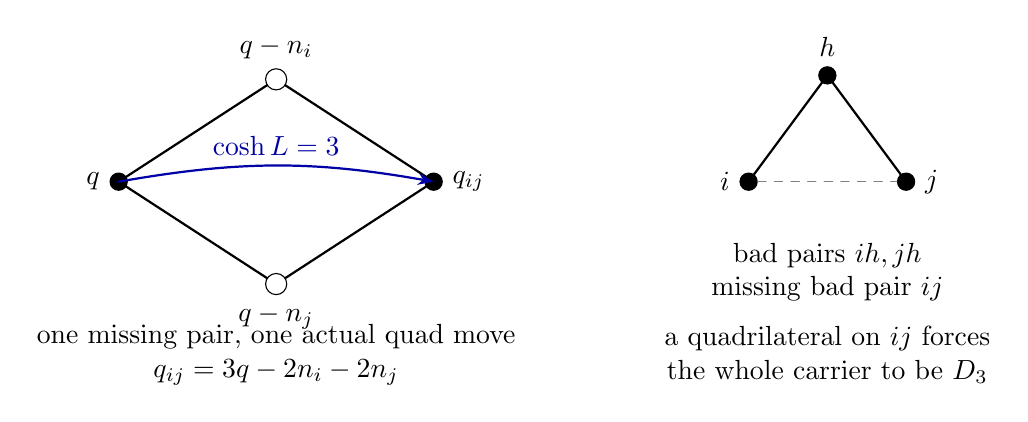
\begin{tikzpicture}
 \coordinate(q) at(-2,0); \coordinate(p) at(2,0);
 \coordinate(ui) at(0,1.3); \coordinate(uj) at(0,-1.3);
 \draw[wall] (q)--(ui)--(p)--(uj)--cycle;
 \node[finite,label=left:\(q\)] at(q){};
 \node[finite,label=right:\(q_{ij}\)] at(p){};
 \node[ideal,label=above:\(q-n_i\)] at(ui){};
 \node[ideal,label=below:\(q-n_j\)] at(uj){};
 \draw[move,bend left=10] (q) to node[above]{\(\cosh L=3\)}(p);
 \node[align=center] at(0,-2.2){one missing pair, one actual quad move\\
 \(q_{ij}=3q-2n_i-2n_j\)};
 \begin{scope}[xshift=7cm]
  \node[finite,label=left:\(i\)] (i) at(-1,0){};
  \node[finite,label=right:\(j\)] (j) at(1,0){};
  \node[finite,label=above:\(h\)] (h) at(0,1.35){};
  \draw[wall] (i)--(h)--(j); \draw[faint] (i)--(j);
  \node[align=center] at(0,-1.15)
   {bad pairs \(ih,jh\)\\missing bad pair \(ij\)};
  \node[align=center] at(0,-2.2)
   {a quadrilateral on \(ij\) forces\\the whole carrier to be \(\Dthree\)};
 \end{scope}
\end{tikzpicture}
\caption{A symmetric quad and its induced-path carrier. The left
panel is an incidence drawing of a hyperbolic two-face; the right is
a graph on directions. The conclusion requires an actual
quadrilateral, not just an induced path in the corner graph.}
\label{fig:quad}
\end{figure}

\subsection{Symmetric multiplicity and the exact missing-path error}
The two cross-wall identities are
\[
 q_{ij}-R_i-n_\ell=q-n_i-n_\ell,\qquad
 q_{ij}-R_j-n_\ell=q-n_j-n_\ell
 \quad(\ell\notin\{i,j\}).
\]
Thus the common bad-neighbor set of the missing pair is identical at
both ends. If it has size \(d_{ij}\), assign the one undirected quad
move weight \(d_{ij}/2\). Several \(\Dthree\) carriers share this
one quad; this weight retains their multiplicity without inventing
separate opposite vertices.

At \(q\), let \(t\) count triangles of \(G_q\), \(b_i\) their
incidences, \(P\) induced two-edge paths, and \(c_i\) such paths in
which \(i\) is an endpoint of the missing pair. Call a path
\emph{backed} if its three-face is \(\Dthree\), equivalently
if its missing pair is the actual symmetric quadrilateral. Use
\(P_b,c_i^b\) for these counts. Actual \(\Pthree\) moves of
weight one and the preceding quad weights have row displacement
\begin{equation}\label{eq:Dactual}
 D_{\rm act}(q)=(t+P_b)q-\sum_i(b_i+c_i^b)n_i,\qquad
 \sum_qD_{\rm act}(q)=0.
\end{equation}
The hypothetical field that backs every path is
\[
 D_{\rm full}(q)=(t+P)q-\sum_i(b_i+c_i)n_i.
\]
If \(M=P-P_b\), then
\begin{equation}\label{eq:error}
 D_{\rm full}-D_{\rm act}=Mq-\sum_i c_i^{\rm miss}n_i,\quad
 \sum_i c_i^{\rm miss}=2M,\quad
 \lVert c^{\rm miss}\rVert_2\le\sqrt2\,M.
\end{equation}
The last bound adds the length-\(\sqrt2\) endpoint vectors of the
missing paths.

Even the full field need not be causal for an arbitrary graph. For
\(K_8\sqcup K_2\sqcup K_2\), \(t=56,P=0\), but its spatial
square is \(8\cdot21^2=3528>56^2\).
No realization by an actual polytope is asserted. Conversely the
graph \(K_5\) joined to seven independent vertices has
\[
 t=80,\quad b=(34^5,10^7),\quad P=105,\quad c=(0^5,30^7).
\]
The triangle field is spacelike since \(6480>80^2\); the full
field is timelike since \(16980<185^2\).
This explains the value of actual quad moves while also displaying
the gap in a universal causal argument.

\section{A second conditional dimension-eight theorem}
\begin{theorem}\label{thm:ideal_edges8}
Suppose \(P\) has a finite vertex, has no finite--finite edges
anywhere, and every three-face satisfies \(\nuu\le11\). Then
\(n\le8\).
\end{theorem}
\begin{proof}
Consider a three-face with \(\nuu=11\). Equations
\eqref{eq:Euler3} give \(p=4s-26\). Since every edge at a
finite vertex ends at a cusp, \(3p\le4c\). Together with
\(c=11-s\) and \(p\ge0\), this forces
\((s,c,p)=(7,4,2)\). Its \(22\) polygon corners require six
triangles and one quadrilateral. Every triangle has at most one finite
corner, and each finite vertex belongs to at most two bad triangles,
since three would force \(\Pthree\). The six finite polygon
corners therefore put both finite vertices in the quadrilateral.
They are opposite because no finite--finite edge is permitted.
The other polygons are four bad and two ideal triangles.
Proposition~\ref{prop:common} identifies \(\Dthree\).
Among the smaller faces, \(\Qeight,\Rseven\) have
finite--finite edges and are excluded. Thus every three-face is
\(\Pthree\) or \(\Dthree\).

At each finite corner, every three-subset of \(G_q\) is a triangle
or a two-edge path. The missing edges consequently form a matching,
of size \(0\le r\le\lfloor n/2\rfloor\). Every missing pair
is an actual symmetric quad. For this theorem count each such quad
once with weight \(1/2\), independent of its number of carriers,
and count each \(\Pthree\) with weight one.
Their displacement sum is undirected. Its positive time coefficient
and its two spatial coefficients are
\[
 a=\bin n3-r(n-3),\quad
 b_{\rm un}=\bin{n-1}{2}-r,\quad
 b_{\rm pair}=\bin{n-2}{2}-r+2.
\]
The first spatial type occurs \(n-2r\) times, and the second \(2r\)
times. For example a triangle is removed once for each matching edge
it contains; each quad displacement restores time one and one spatial
unit at its two endpoints. Expanding
\(a^2-(n-2r)b_{\rm un}^2-2rb_{\rm pair}^2\) gives
\[
\begin{array}{c|l}
 n&\text{causal margin}\\ \hline
 9&7r^2+6r\\
 10&1440-168r+15r^2\\
 11&4950-488r+25r^2\\
 12&12100-1008r+37r^2 .
\end{array}
\]
The first is nonnegative, and the other three are positive on the
allowed interval, with minima \(975,3135,7384\).
Every row is nonzero future causal, contradicting cancellation.
This excludes dimensions \(9\)--\(12\). If \(n>12\), take a
twelve-face through a finite vertex. It inherits the absence of
finite--finite edges and the same three-face condition, giving the
same contradiction. Thus \(n\le8\).
\end{proof}

Both global hypotheses in this theorem matter. An all-ideal-direction
corner or component alone does not show that other finite vertices
of a three-face have no finite--finite edges. The theorem therefore
cannot be substituted into the unrestricted mixed problem.

\section{Universal carrier charges and maximum-height restrictions}
\subsection{Missing paths have a quantified carrier cost}
For a non-\(\Pthree\) three-face let \(Z\) count its finite
corners with induced-path direction graph. At each such corner the
three neighboring vertices are distinct cusps and two incident facets
are bad triangles. Distinct bad triangles use distinct ideal--ideal
edges by Lemma~\ref{lem:attachment}. Thus
\[
 E_{FI}\ge3Z,\qquad E_{II}\ge2Z,\qquad
 4c=E_{FI}+2E_{II}\ge7Z,\qquad p\ge Z.
\]
Together with \(p+4c=2\nuu-4\), these give
\begin{equation}\label{eq:Z}
 4Z\le\nuu-2.
\end{equation}
For integer \(\nuu\ge12\), \(Z\le2(\nuu-11)\):
at twelve the integer bound is \(Z\le2\); for larger \(\nuu\)
the inequality follows directly.

The remaining sum-eleven case can be determined exactly at an
induced-path corner. Its three cusp neighbors give \(c\ge3\);
\(p=4s-26\) then leaves \((s,c,p)=(7,4,2)\) or \((8,3,6)\).
The first is \(\Dthree\), since the chosen corner already uses
all its finite degree and no edge can join the two finite vertices.
It is backed. In the second all cusps neighbor the chosen corner.
Any edge between two of those cusps lies in their common face with
that finite corner: simplicity in dimension three puts the two
incident edges in a polygon containing the corner and both cusps,
and an edge between the cusps forces that polygon to be exactly
their triangle. Thus the ideal--ideal edge graph is precisely the
two-edge path. Consequently
\[
 E_{II}=2,\quad E_{FI}=8,\quad E_{FF}=5.
\]
There is at most one such induced-path corner, since another would
reuse an ideal--ideal edge in bad triangles, triggering attachment.

\begin{theorem}\label{thm:charge}
Let
\[
 E_{12}=\sum_{\nuu(F)\ge12}(\nuu(F)-11),
\]
and let \(e_{FF}\) count finite--finite edges of the ambient
polytope. With the universal actual move set
\eqref{eq:Dactual}, its missing-path counts satisfy
\begin{equation}\label{eq:charge}
 \sum_q M(q)\le2E_{12}
       +\frac15\bin{n-1}{2}e_{FF}.
\end{equation}
\end{theorem}
\begin{proof}
No carrier with sum at most ten has an induced-path corner.
The sum-eleven unbacked type just described pays its at most one
missing path with five finite--finite edges. Larger carriers are
bounded by \eqref{eq:Z}. Finally each ambient finite--finite edge
belongs to \(\bin{n-1}{2}\) three-faces.
\end{proof}

One may keep the finite-edge incidences of just the
\((s,c,p)=(8,3,6)\) carriers, making the second term sharper.
A companion count bounds all finite corners with three ideal edges
in three-faces other than \(\Pthree,\Dthree\):
\begin{equation}\label{eq:companion}
 N_{\rm noncanonical}\le
 5E_{12}+\frac23\bin{n-1}{2}e_{FF}.
\end{equation}
Here is the additional argument. At sum eleven the type is again
\((8,3,6)\). Its ideal--ideal graph has \(j=0,1,2\) edges:
if such a corner exists, every ideal--ideal edge joins two of its
three cusp neighbors and hence is a bad triangle there; three would
give \(\Pthree\). For \(j\ge1\), attachment permits at most
one such corner; for \(j=0\), three would produce a planar
\(K_{3,3}\), impossible by Euler's bipartite edge bound.
There are \(3+j\) finite--finite edges, so the number is at most
\((2/3)E_{FF}\). For larger carriers the number \(A_3\) of
these corners satisfies \(3A_3\le4c,\ p\ge A_3\), whence
\(A_3\le(\nuu-2)/2\le5(\nuu-11)\).
This proves \eqref{eq:companion}.

\subsection{Maximum height is a local hypothesis}
Fix any future unit \(u\), and choose a finite vertex \(q\) maximizing
\(H(q)=-\ip{u}{q}\) among all finite vertices. Its coordinates
\(p_i=-\ip{u}{n_i}/H(q)\) satisfy \(\sum p_i^2<1\).
Every actual move gives a necessary inequality:
\begin{align}
 \sum_{i\in S}p_i&\ge1
       &&\text{for every actual \(\Pthree\) triple},\label{eq:maxtri}\\
 p_i+p_j&\ge1
       &&\text{for every actual symmetric quad pair},\label{eq:maxquad}\\
 p_i&\ge\sqrt2-1
       &&\text{for every finite edge of \(\cosh L=\sqrt2\)}.
       \label{eq:maxedge}
\end{align}
These follow by applying \(H(q')\le H(q)\) to the displayed
Lorentz move formulas; they do not require other carriers to be small.

Two disjoint quad pairs would use squared norm at least one, so
the backed missing pairs form an intersecting family: a star or a
triangle. Indeed two intersecting pairs \(ab,ac\) force any pair
avoiding \(a\) to be \(bc\), after which no fourth pair is possible.
A quad pair disjoint from two disjoint \(\Pthree\) triples is
also impossible, by norm cost \(1/2+1/3+1/3>1\). So is a
disjoint quad pair, triple and short finite-edge direction:
\[
 \frac12+\frac13+(\sqrt2-1)^2>1.
\]
The last strict inequality is equivalent to \(289>288\).
A backed pair cannot have a \(K_5\) among its common bad neighbors:
summing the ten triple constraints on those five directions gives
norm cost at least \(5/9\), disjoint from the pair's \(1/2\).

\begin{figure}[ht]
\centering
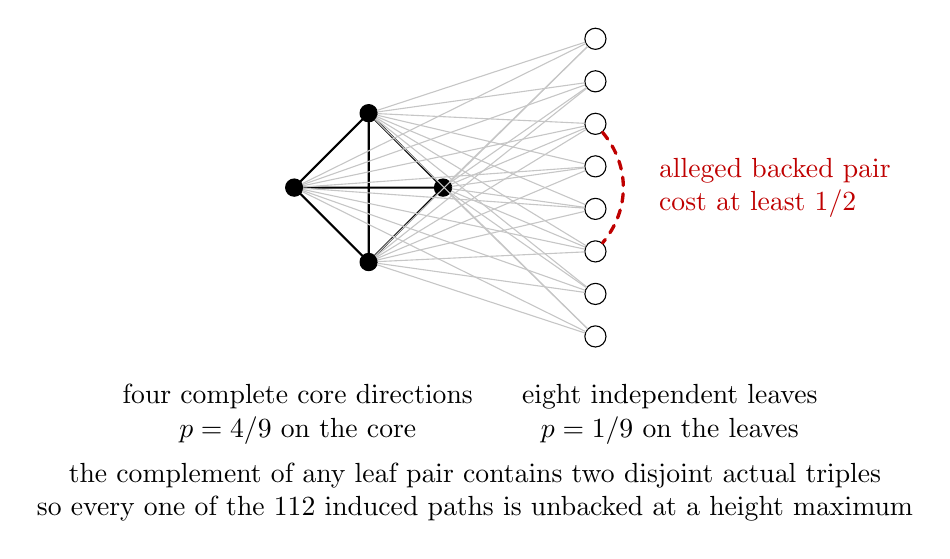
\begin{tikzpicture}[scale=.9]
 \foreach \a/\name in {90/a,180/b,270/c,0/d}{
  \node[finite] (\name) at(\a:1.05){};
 }
 \draw[wall] (a)--(b)--(c)--(d)--(a)--(c) (b)--(d);
 \foreach \j in {1,...,8}{
  \node[ideal] (l\j) at(3.2,{2.1-.6*(\j-1)}){};
  \foreach \name in {a,b,c,d} \draw[gray!45] (\name)--(l\j);
 }
 \draw[red!75!black,very thick,dashed,bend left=40]
  (l3) to node[right=9pt,align=left]{alleged backed pair\\cost at least \(1/2\)}(l6);
 \node[align=center] at(-1,-3.2){four complete core directions\\
 \(p=4/9\) on the core};
 \node[align=center] at(4.25,-3.2){eight independent leaves\\
 \(p=1/9\) on the leaves};
 \node[align=center] at(1.5,-4.3)
 {the complement of any leaf pair contains two disjoint actual triples\\
 so every one of the \(112\) induced paths is unbacked at a height maximum};
\end{tikzpicture}
\caption{A local defect forced by maximum height. The drawing is a
corner graph \(K_4\) joined to an independent set of eight directions,
not a proposed polytope. Its triple constraints admit norm \(8/9\),
but no missing pair can be backed by an actual symmetric quad.}
\end{figure}

For that example the core coordinates \(4/9\) and leaf coordinates
\(1/9\) satisfy all \(\Pthree\) constraints with squared norm
\(8/9<1\). Yet a backed pair would be two leaves, whose complement
contains two disjoint triples using two core vertices each.
Thus all \(4\bin82=112\) induced paths are unbacked at such a
maximum vertex. Theorem~\ref{thm:charge} identifies the possible
carriers of this defect. This does not imply that every finite vertex
is a height maximum for some future \(u\), nor does it bound the
unweighted global triangle average.

\section{What the transport argument still needs}
The actual moves and carrier charges hold without arithmetic
restrictions or a finite census of high-dimensional polytopes.
Nevertheless \eqref{eq:error} is not presently small enough to
force a contradiction in every dimension-twelve system, and
\(D_{\rm full}\) itself can be spacelike on abstract graph data.
One must exploit additional geometric restrictions on those data,
or obtain stronger capacity bounds along actual edges and carriers.
The local triangle-count question at a maximum vertex is not settled
here. No claim concerning its global average is made.

Theorems~\ref{thm:small8} and \ref{thm:ideal_edges8} exclude whole
restricted carrier systems, not arbitrary mixed polytopes.
Theorem~\ref{thm:fraction} quantifies a necessary defect in dimension
twelve. The component theorem and quad charges retain actual
adjacency information that scalar incidence relaxations omit.
All these conclusions coexist with the unchanged unconditional
mixed ceiling twelve.

\section*{Proof and reproduction record}
This manuscript consolidates reviewed research packets without changing
their frozen sources. The complete file-level map is
\file{docs/right_angled_mixed_opposition_transport_proof_map.md}.
The small-carrier theorem has a nine-row exact
\(\mathbb Q(\sqrt2)\) checker. The excess-fraction theorem has a
\(178\)-box rational interval checker. The opposition moment constants
have separate rational polynomial checkers. The actual-support and
symmetric-quad results have independent written mathematical reviews.
These scopes are separate: arithmetic replay does not formalize the
universal hyperbolic geometry, and a TeX build checks typesetting only.
The author of this translation ran no checker or TeX process while
writing this source; other agents' coordinated jobs are separate.

\begin{thebibliography}{9}
\bibitem{PV}
L.~Potyagailo and E.~Vinberg,
\emph{On right-angled reflection groups in hyperbolic spaces},
Commentarii Mathematici Helvetici \textbf{80} (2005), 63--73.
\href{https://ems.press/content/serial-article-files/43032}{Publisher text}.
\end{thebibliography}
\end{document}
